% Chapter 3: Cloud Backend
\section{Serverless Cloud Architecture}

\subsection{AWS Backend Design}
The cloud backend uses AWS serverless services for automatic scaling, pay-per-use pricing, and zero server management.

\begin{table}[H]
\centering
\caption{Lambda Function Configuration}
\label{tab:lambda_config}
\begin{tabular}{llcc}
\toprule
\textbf{Function} & \textbf{Deploy} & \textbf{Memory} & \textbf{Timeout} \\
\midrule
HealthDataIngestion & Zip & 512MB & 30s \\
HealthAnomalyInference & Container & 1024MB & 30s \\
HealthReadMetrics & Zip & 256MB & 30s \\
HealthSnsToExpo & Zip & 256MB & 30s \\
\bottomrule
\end{tabular}
\end{table}

\subsection{API Endpoints}
REST API via API Gateway with API key authentication (\texttt{X-API-Key} header): POST \texttt{/health-data/ingest} (data ingestion), GET \texttt{/health-data/sync} (read metrics), POST \texttt{/notifications/register} (push token registration).

\subsection{DynamoDB Schema}
Two tables: \textbf{HealthMetrics} (PK: userId, SK: timestamp; stores HR, steps, calories, anomalyReasons) and \textbf{HealthPushTokens} (PK: userId; stores deviceId, expoPushToken, TTL: 90 days).

\subsection{Cloud Backend Performance}

\begin{figure}[H]
\centering
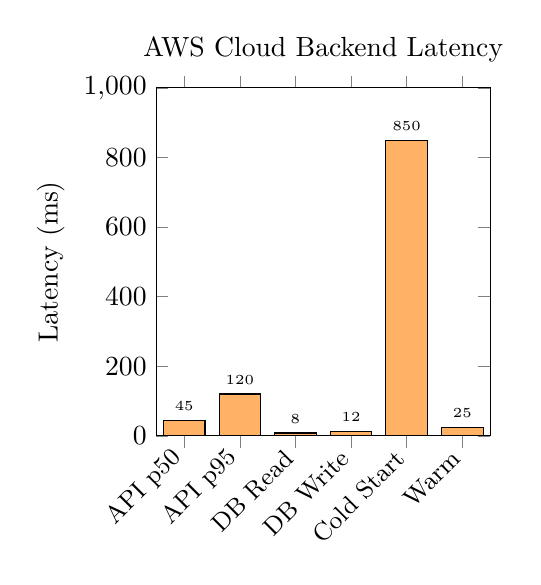
\begin{tikzpicture}
\begin{axis}[
    ybar, bar width=15pt, ylabel={Latency (ms)},
    symbolic x coords={API p50, API p95, DB Read, DB Write, Cold Start, Warm},
    xtick=data, x tick label style={rotate=45, anchor=east, font=\small},
    ymin=0, ymax=1000, nodes near coords,
    width=0.48\textwidth, height=6cm,
    title={AWS Cloud Backend Latency},
    every node near coord/.append style={font=\tiny},
]
\addplot[fill=orange!60] coordinates {
    (API p50, 45) (API p95, 120) (DB Read, 8) (DB Write, 12) (Cold Start, 850) (Warm, 25)
};
\end{axis}
\end{tikzpicture}
\caption{Cloud backend latency performance.}
\label{fig:cloud_latency}
\end{figure}

\subsection{Alert Delivery Pipeline}

\begin{table}[H]
\centering
\caption{End-to-End Alert Delivery Timing}
\label{tab:alert_pipeline}
\begin{tabular}{lcc}
\toprule
\textbf{Stage} & \textbf{Latency (ms)} & \textbf{Cumulative} \\
\midrule
API Gateway routing & 15 & 15 \\
Ingestion Lambda & 45 & 60 \\
DynamoDB write & 12 & 72 \\
Inference invocation & 120 & 192 \\
SNS publish & 30 & 222 \\
SNS-to-Expo Lambda & 200 & 422 \\
Expo push delivery & 500--2000 & 922--2422 \\
\midrule
\textbf{Total (warm)} & & \textbf{$\sim$1--2.5s} \\
\bottomrule
\end{tabular}
\end{table}

\subsection{Cost Analysis}

\begin{figure}[H]
\centering
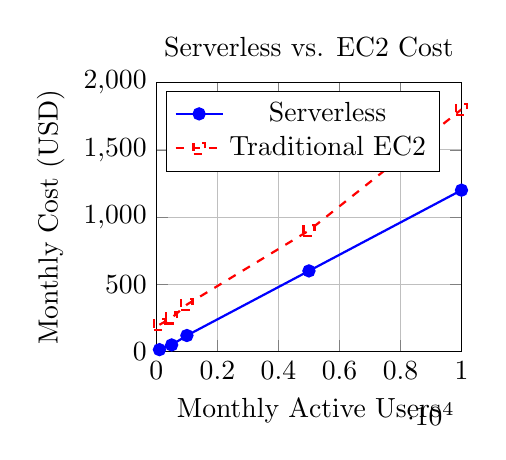
\begin{tikzpicture}
\begin{axis}[
    xlabel={Monthly Active Users}, ylabel={Monthly Cost (USD)},
    xmin=0, xmax=10000, ymin=0, ymax=2000,
    legend pos=north west, grid=major,
    width=0.45\textwidth, height=5cm,
    title={Serverless vs. EC2 Cost},
]
\addplot[thick, blue, mark=*] coordinates {
    (100, 15) (500, 50) (1000, 120) (5000, 600) (10000, 1200)
};
\addlegendentry{Serverless}
\addplot[thick, red, dashed, mark=square] coordinates {
    (100, 200) (500, 250) (1000, 350) (5000, 900) (10000, 1800)
};
\addlegendentry{Traditional EC2}
\end{axis}
\end{tikzpicture}
\caption{Cost comparison at varying user scales.}
\label{fig:cost}
\end{figure}
